\documentclass[aspectratio=43,t]{beamer}

% Colors
\usepackage{color}
\definecolor{mainorange}{HTML}{EC811B}
\definecolor{lightgrey}{HTML}{888888}
\definecolor{librepcb}{RGB}{41,214,130}

% Syntax highlighting
\usepackage{minted}
\usepackage{alltt}
\newcommand\hi[1]{{\color{mainorange} \textbf{#1}}}

% Directory trees
\usepackage{dirtree}

% Tikz
\usepackage{tikz}
\usepackage{tikzsymbols}
\usetikzlibrary{calc}
\usetikzlibrary{positioning}
\usetikzlibrary{fit}
\usetikzlibrary{matrix}
\usetikzlibrary{shapes, shapes.callouts}
\usetikzlibrary{shadows}
\usetikzlibrary{arrows, arrows.meta}
\usetikzlibrary{backgrounds}
\pgfdeclarelayer{background}
\pgfdeclarelayer{foreground}
\pgfsetlayers{background,main,foreground}
\tikzstyle{lpbox}=[rectangle, draw=black, rounded corners, fill=librepcb, drop shadow,
                   text centered, anchor=north, text=white]
\tikzstyle{lpline}=[]
\tikzstyle{lparrow}=[lpline, -{Stealth}]
\tikzstyle{lparrow2}=[lpline, {Stealth}-{Stealth}]

% Various packages
\usepackage{multirow}
\usepackage{array}
\usepackage[framemethod=TikZ]{mdframed}
\usepackage{fontawesome}

% Theme
\usetheme[%
  sectionpage=none,
  subsectionpage=none,
  numbering=fraction,
  progressbar=foot,
]{metropolis}

% Customization
\setbeamertemplate{section in toc}[sections numbered]
\setbeamerfont{title}{size=\fontsize{30}{30}}
\setbeamerfont{block title}{size=\large}
\newcommand\sep{\textcolor{lightgrey}{\rule{\linewidth}{0.05mm}}}

% Meta
\title{LibrePCB}
\subtitle{A new, powerful and intuitive EDA tool for everyone}
\date{\today}
\author{Urban Bruhin}
\institute{}

\begin{document}

% ----------------------------------------------------------------- %

\maketitle

% ----------------------------------------------------------------- %

%\begin{frame}[plain,noframenumbering]
%	\frametitle{Table of Contents}
%	\setcounter{tocdepth}{1}
%	\tableofcontents
%\end{frame}

% ----------------------------------------------------------------- %

\section{About LibrePCB}

\begin{frame}{\secname}
  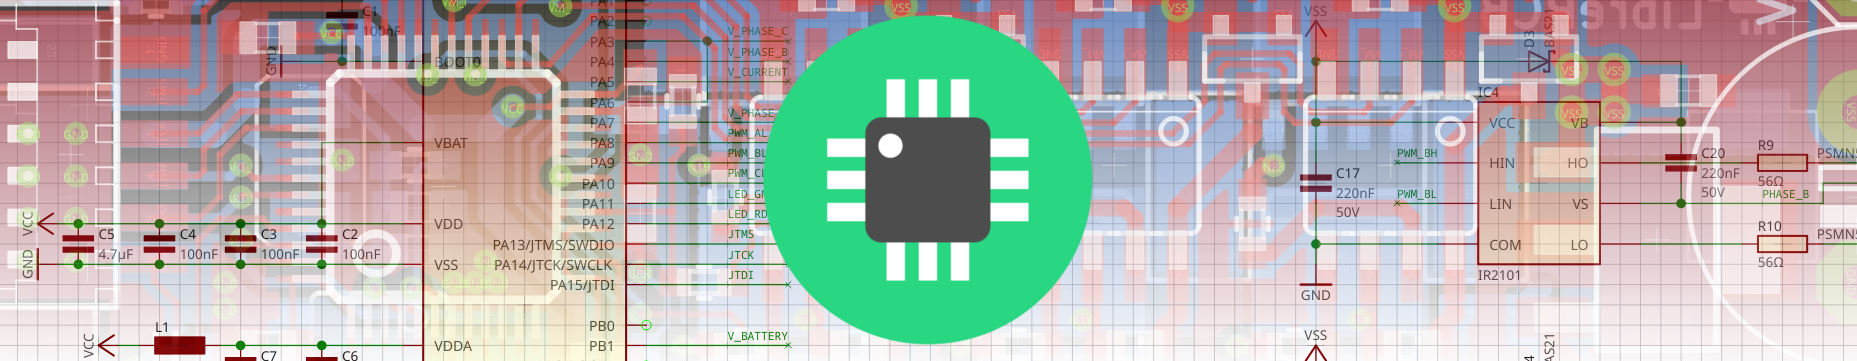
\includegraphics[width=\linewidth]{images/about_header.png} \linebreak\linebreak
  \textbf{Free/OpenSource EDA Suite}
  \begin{itemize}
    \item Multiplatform \faLinux\ \faApple\ \faWindows\
    \item Written from scratch in C++11/Qt5
    \item Development started in February 2013
    \item Website: \url{http://librepcb.org/}
    \item GitHub: \url{https://github.com/LibrePCB/LibrePCB}
  \end{itemize}
\end{frame}
\section{File Format Extensibility}

\begin{frame}{\secname}
  \textbf{Problem}
  \begin{itemize}
    \item File format of other tools were not designed for extensibility
  \end{itemize}
  
  \pause
  
  \textbf{Result}
  \begin{itemize}
    \item Missing or broken support for 3D models
    \item Missing or broken support for SPICE models
    \item Not ready for future extensions
  \end{itemize}
\end{frame}

\begin{frame}{\secname}
  \textbf{Solution}
  \begin{itemize}
    \item 1 entity = 1 directory
  \end{itemize}
  
  \pause
  
  \begin{center}
    \color{blue}
    \vspace*{-\baselineskip}\leavevmode % reduce space
    \begin{tikzpicture}[node distance=5mm, hint/.style={rectangle callout, fill=librepcb!30, text=black, rounded corners}]
      % uuid
      \node (dir) [] {
        \large\faFolderOpenO
      };
      \node (uuid) [anchor=west] at (dir.east) {
        \large\texttt{2d9ba47b-3ff1-44db-aa4e-0bfec1f12ea8}
      };
      \node [hint, above right=of uuid, anchor=south east, callout absolute pointer=(uuid.north)] {
        Directory name = entity UUID
      };
      
      % version file
      \node (file1) [anchor=north west] at (dir.south east) {
        \large\faFileTextO\ \large\texttt{.librepcb-pkg}
      };
      \draw (dir.south) |- (file1.west);
      \node [hint, below right=5mm and 2cm of file1.north east, anchor=north west, callout absolute pointer=(file1.east), text width=4.5cm] {
        Plain text file\\
        $\bullet$ Forward compatible\\
        $\bullet$ Filename = entity type\\
        $\bullet$ Content = format version 
      };
      
      % entity file
      \node (file2) [anchor=north west] at (file1.south west) {
        \large\faFileTextO\ \large\texttt{package.lp}
      };
      \draw (dir.south) |- (file2.west);
      \node [hint, below right=17mm and 8mm of file2, anchor=north west, callout absolute pointer=(file2.east), text width=4.5cm] {
        S-Expression file containing the actual entity data
      };
      
      % 3dmodel
      \onslide<3->{
        \node (file3) [anchor=north west] at (file2.south west) {
        \large\faFileImageO\ \large\texttt{3dmodel.wrl}};
        \draw (dir.south) |- (file3.west);
      }
      
      % step model
      \onslide<4->{
        \node (file4) [anchor=north west] at (file3.south west) {
        \large\faFileImageO\ \large\texttt{3dmodel.step}};
        \draw (dir.south) |- (file4.west);
      }
      
      % spice model
      \onslide<5->{
        \node (file5) [anchor=north west] at (file4.south west) {
        \large\faFileTextO\ \large\texttt{spice.mod}};
        \draw (dir.south) |- (file5.west);
      }
    \end{tikzpicture}
  \end{center}
\end{frame}
\section{Self-Contained Projects}

\begin{frame}{\secname}
  \textbf{Problem}
  \begin{itemize}
    \item Projects depend on information stored outside the project
    \begin{itemize}
      \item Library entities, settings, fonts, ...
    \end{itemize}
  \end{itemize}
  
  \pause
  
  \textbf{Result}
  \begin{itemize}
    \item Projects are not portable (e.g. \textit{"Library not found"} errors)
    \item Generated production data is not reproducible
    \item Source code is harder to maintain (more changes are breaking)
  \end{itemize}
  
  \pause
  
  \textbf{Solution}
  \begin{itemize}
    \item Embed as much information as possible into projects
    \begin{itemize}
      \item Library entities (forced, not optional)
      \item All relevant settings
      \item Fonts \textit{(work in progress...)}
    \end{itemize}
  \end{itemize}
\end{frame}
\section{Version Control Systems}

\begin{frame}{\secname}

  \begin{columns}[onlytextwidth]
    \begin{column}{\textwidth-3.5cm}
      \textbf{Problem}
      \begin{itemize}
        \item Important and unimportant data mixed
        \item Unclear which files to version control
      \end{itemize}

      \pause

      \textbf{Result}
      \begin{itemize}
        \item Local changes even if nothing modified
        \item Very large and opaque diffs/commits
        \item Important files accidentally ignored
      \end{itemize}

      \pause

      \textbf{Solution}
      \begin{itemize}
        \item Many small files for higher granularity
        \item Unimportant data strictly separated
        \item Automatic creation of \texttt{.gitignore}
      \end{itemize}
    \end{column}

    \hfill

    \begin{column}{3.5cm}
      \color{blue}\dirtree{%
        .1 MyProject.
        .2 .gitignore.
        .2 boards.
          .3 default.lp.
        .2 core.
          .3 circuit.lp.
          .3 erc.lp.
          .3 settings.lp.
%        .2 library.
%          .3 \dots.
        .2 output.
          .3 \dots.
        .2 schematics.
          .3 power.lp.
          .3 logic.lp.
        .2 user.
          .3 \dots.
      }
    \end{column}
  \end{columns}
\end{frame}

\section{Version Control Systems}

\begin{frame}[fragile]{\secname}
  \begin{minted}[baselinestretch=.8,style=trac]{diff}
--- a/test.kicad_pcb
+++ b/test.kicad_pcb
@@ -3,7 +3,7 @@
   (general
     (no_connects 0)
-    (area 41.834999 87.554999 233.755001 153.745001)
+    (area 20.171999 28.969758 233.755001 157.374234)
     (drawings 4)
@@ -21,7 +21,7 @@
     (36 B.SilkS user)
-    (37 F.SilkS user)
+    (37 F.SilkS user hide)
     (38 B.Mask user hide)
@@ -62,7 +62,7 @@
     (aux_axis_origin 0 0)
-    (visible_elements FFFC4601)
+    (visible_elements FFFC4609)
     (pcbplotparams
       (layerselection 0x00030_80000001)\end{minted}
  
  \scriptsize{
    KiCad 4.0.2+dfsg1-stable:
    zoom around,
    hide "F.SilkS",
    show "Through Via"
  }
\end{frame}

\begin{frame}[noframenumbering]{\secname}
  \textbf{Problem}
  \begin{itemize}
    \item Files are \textbf{not really} human readable
  \end{itemize}

  \pause

  \textbf{Result}
  \begin{itemize}
    \item Diffs are very hard to understand
    \item Limited use of version control systems
  \end{itemize}

  \pause

  \textbf{Solution}
  \begin{itemize}
    \item Don't just consider text-based file formats as human readable!
    \item Control every tiny detail of the generated files
    \item Consider opaque parts of files as bugs and fix them
  \end{itemize}
\end{frame}

\section{Contributing}

\begin{frame}{\secname}
  \begin{centering}
    \bigskip \bigskip
    \textbf{\Huge Contributors welcome!}\\
    \bigskip \bigskip
    {\footnotesize \url{https://github.com/LibrePCB/LibrePCB/blob/master/CONTRIBUTING.md}}\\
    {\footnotesize IRC: \texttt{\#librepcb} on Freenode}\\
  \end{centering}
  \textbf{\Large
    \begin{itemize}
      \centering
      \item Participate in issues
      \item Open pull requests
      \item Improve documentation
      \item Donate (Patreon, GitHub Sponsors, \dots)
    \end{itemize}
  }
\end{frame}


% ----------------------------------------------------------------- %

{
\setbeamertemplate{footline}{}
\begin{frame}[standout]
	\begin{centering}
	{\Huge Thank you!}\\
	{\normalsize \url{http://librepcb.org}}\\
	\end{centering}
\end{frame}
}

% ----------------------------------------------------------------- %

\end{document}
